\renewcommand\thetable{\arabic{chapter}-\arabic{table}}
%\renewcommand\thefigure{\arabic{chapter}-\arabic{figure}} 
\chapter{結論與未來展望}
\label{cha:conclusions}


\section{結論}

教育部所主持的「加速高中職及國中小老舊校舍及相關設備補強整建計畫」以及其相關的後續計畫,在執行上和一般的計畫一樣會受到預算的限制,但是此一計畫的預算限制直接的影響到能夠改善多少校舍的耐震能力,因此如何有效的估計校舍詳細評估、補強的預算需求,並正確的挑選出應該優先處理的校舍對於學生的生命安全關係重大,然而實際上校舍補強的正確經費是在計畫非常後期才會得到,因此在每個年度的一開始,計畫的執行人員都要透過經驗公式來推估帶評估的校舍需要多少經費來評估和補強,雖然此一經驗公式也有一定程度的可靠度,但是其尚缺乏理論支撐。

需要補強的校舍在得知實際的補強經費之前,會先經過初步評估、詳細評估和補強設計幾個階段的作業,然後才是實際的補強施工,本研究目前的成果也是分佈在此一程序上的不同位置,包括了初步評估的~$Is$~值關係模型、詳細評估的~$CDR$~值關係模型、詳細評估的破壞構件關係模型、以及最後的校舍補強經費關係模型。

\begin{figure}[hbtp]
  \begin{center}
    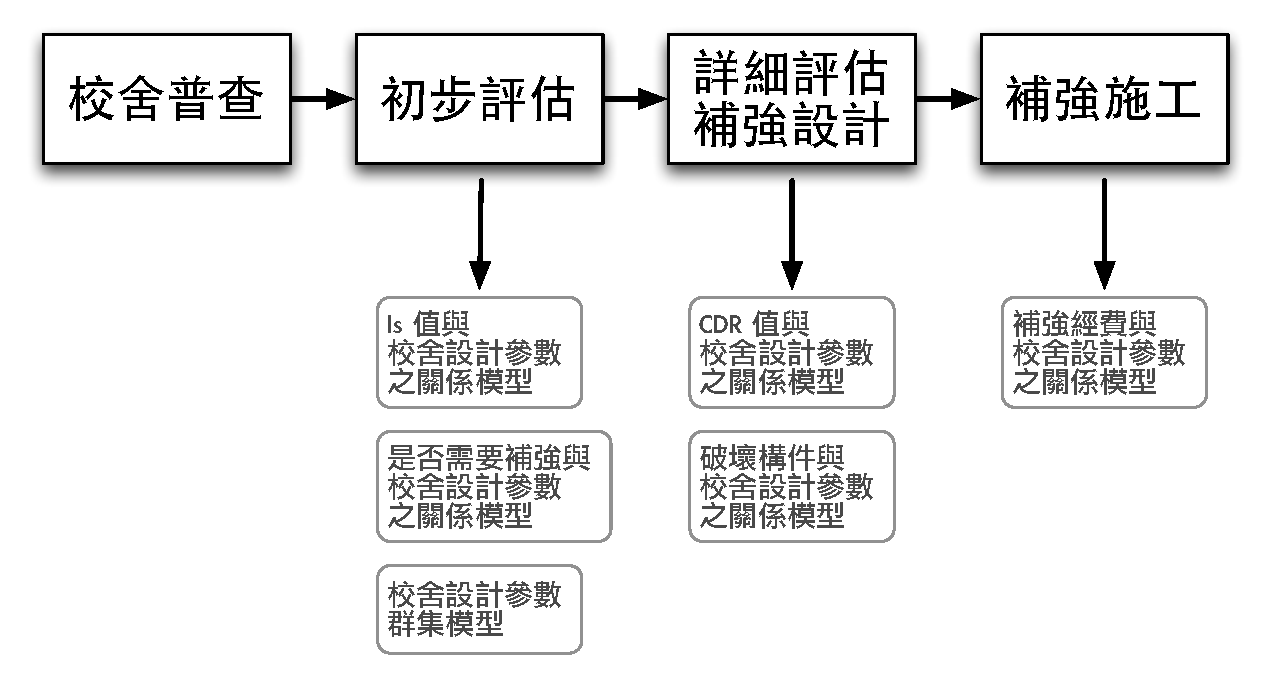
\includegraphics[width=1.0\textwidth]{figures/survey-flow-con.pdf}
    \caption{評估流程與資料探勘模型} 
    \label{fig:FLOW-con}
  \end{center}
\end{figure}

\section{未來展望} 

%本論文主要之成果為耐震能力與補強預算相關之知識
%未來發展方向為其他之知識

資料探勘可分為四種知識型態,包括了迴歸、分類、分群、關聯四種,本研究初期依據此四種型態分析設計了數個不同面向的探勘目標:

\begin{description}
  \item[迴歸]
  主要的知識為重要屬性的關係模型,且要為數值類型的屬性,例如校舍的最小破壞地表加速度、耐震能力、補強經費等。
  \item[分類]
  分類探勘類型的知識和迴歸類之知識相似,主要也是用在建立重要屬性的關係模型,其主要差異在於迴歸分析僅能對數值類型之屬性建立模型,而分類分析則僅能對資料數值為集合類之屬性建立模型,目前最主要的分析是校舍是否安全、是否需要補強的分類分析。
  \item[分群]
  分群類型之知識主要在於校舍結構之不同群集,其知識之形式與分類分析有些相似,最大之不同點在於此類模型在訓練建立時,並沒有輸出參數,而是只靠輸入參數間來判斷資料間的相似度ㄋ,例如相似結構形式的校舍群集,組成校舍的結構元件的探勘等。
  \item[關聯]
  關聯類型之知識則包括了校舍結構之設計模式、不同年代校舍之設計特色等。
\end{description}

本研究目前透過資料探勘所得到之知識主要都是以輔助目前的校舍耐震能力補強計畫流程作為出發點,包括了分類形式的校舍是否需要補強與其設計參數之關係模型、迴歸形式的校舍耐震能力與其設計參數之關係模型以及校舍補強經費與其設計參數之關係模型、還有分群形式的校舍群集模型,其在建立耐震能力關係模型時,作為資料前處理輔助用。



在本研究中,建立校舍設計參數與其~$Is$~值之關係模型時,便有使用到此一知識來增進關係模型的品質,後續研究還可以針對這些校舍群集,進一步分析其不同群集之特性,至於關聯形式的知識,本研究目前尚未有可用的知識產出,因此後續的研究方向也包含此一類型知識的探勘與挖掘。


% 資料探勘可分為四種知識型態,包括了迴歸、分類、分群、關聯四種,本研究初期依據此四種型態分析設計了數個不同面向的探勘目標,其中迴歸分析中,主要的知識為重要屬性的關係模型,例如本研究中的耐震能力、補強經費與校舍基本設計參數間之關係模型即為此一類之資料探勘。而分類分析中,目前最主要的分析是校舍是否安全、是否需要補強的分類探勘,即為本研究中所建立之校舍基礎設計參數與是否需要補強間之關係模型。分群類型之知識主要在於校舍結構之不同群集,在本研究中,建立校舍設計參數與其~$Is$~值之關係模型時,便有使用到此一知識來增進關係模型的品質,後續研究還可以針對這些校舍群集,進一步分析其不同群集之特性,至於關聯形式的知識,本研究目前尚未有可用的知識產出,因此後續的研究方向也包含此一類型知識的探勘與挖掘。

\begin{figure}[hbtp]
  \begin{center}
    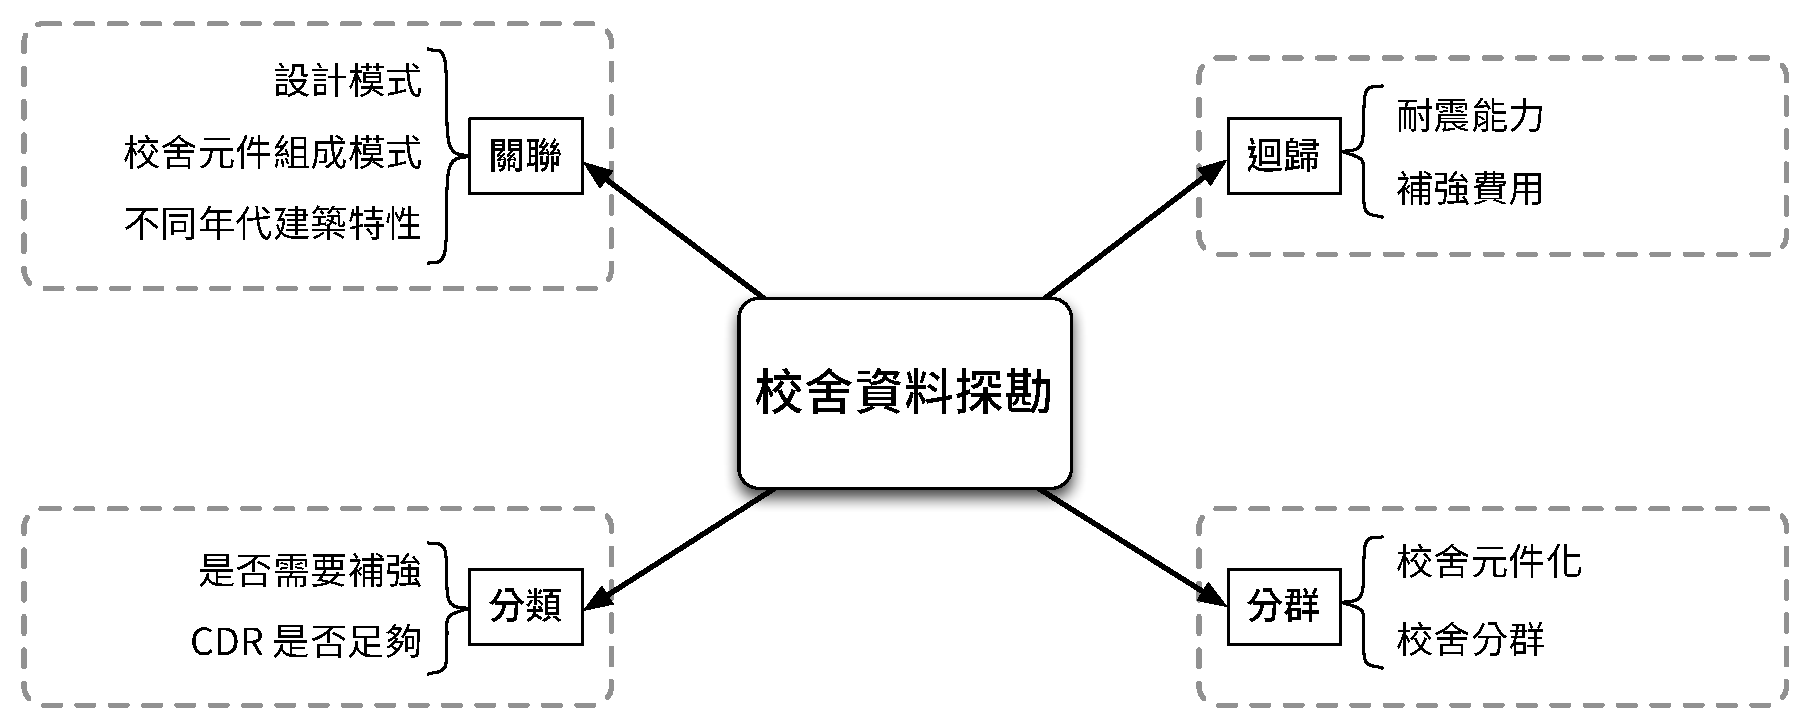
\includegraphics[width=1.0\textwidth]{figures/big-picture.pdf}
    \caption{知識挖掘規劃} 
    \label{fig:bigpicture}
  \end{center}
\end{figure}

另外一個發展方向,則是在~CRISP-DM~流程當中的最後一個步驟,將探勘得到的知識實際回饋到學校校舍及相關設備補強整建計畫上,由於目前探勘得到的知識都還是以數學模型的形式存在,非專業人士難以應用,因此如果可以將這些數學模型轉化成決策支援系統,則可以讓主管機關能夠簡單的得到這些模型的輔助,在校舍長期持續的耐震能力監控上,能夠發揮探勘所得知識的效力。


